
\newpage
\section{CIP biharmonic problem }%
\label{sec:CIP_biharmonic_problem}




\subsection{Strong form of the biharmonic problem}%
\label{sub:strong_form_of_the_biharmonic_equation}

Let $\Omega \subseteq    \mathbb{R} ^d$ be a bounded polygonal domain and $\Gamma $ be its corresponding boundary. Let the biharmonic problem have the form,

\begin{equation}
\label{eq:bi_problem}
\begin{split}
    \Delta^2  u  + \alpha  u  & = f( x)  \quad \text{in } \Omega,   \\
    \partial _{n} u & = g_{1}  \quad \text{on } \partial \Omega,  \\
    \partial _{n} \Delta  u & = g_{2}  \quad \text{on } \partial \Omega .  \\
\end{split}
\end{equation}
Here is $\Delta ^2 = \Delta  \left( \Delta  \right) $ the biharmonic operator, also known as the bilaplacian. We will assume for the strong form that $u \in H^{4}\left( \Omega  \right) $, $\alpha  \in  \mathbb{R} $ and $f, \in L^{2}\left( \Omega  \right)
$. The functions $g_{1},g_{2}: \Omega  \to \mathbb{R}$ are denoted as boundary conditions.

\subsection{  Weak form biharmonic equation in $H^{4}\left( \Omega  \right) $}%
\label{sub:continious_weak_form_of_biharmonic_equation}

\begin{figure}
  \centering
  \begin{minipage}[b]{0.45\textwidth}
    \centering
    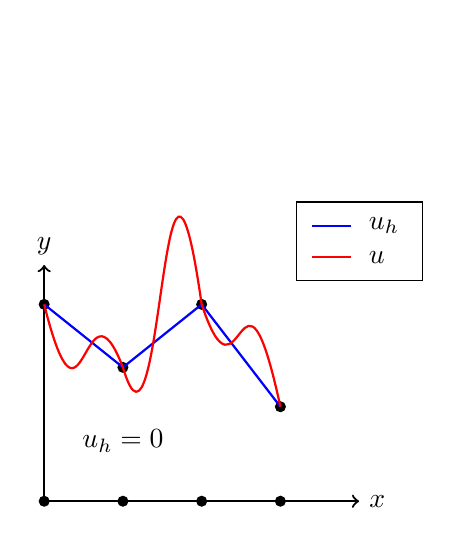
\begin{tikzpicture}
      % Draw x-axis
      \draw[->, thick] (0,0) -- (4,0) node[right] {$x$};
      % Draw y-axis
      \draw[->, thick] (0,0) -- (0,3) node[above] {$y$};

      % Draw nodes at center, A, B, and C with arbitrary y-values
      \foreach \x/\y in {0/2.5, 1/1.7, 2/2.5, 3/1.2} {
        \fill (\x,\y) circle (2pt); % Filled nodes with y-values
        \fill (\x,0) circle (2pt); % Filled circles on x-axis
      }

      % Draw linear interpolation between points
      \draw[blue, thick] (0,2.5) -- (1,1.7) -- (2,2.5) -- (3,1.2);

      \draw[red, thick] (0,2.5) .. controls (0.5,0.5) and (0.5,3) .. (1,1.7) .. controls (1.5,0) and (1.5,6) .. (2,2.5) .. controls (2.5,1) and (2.5,3.5) .. (3,1.2);
      \node at (1,0.5) [above] {$\jump{ u_{h} } = 0$};

      \draw (3.2,2.8) rectangle (4.8,3.8); % Legend box
      \draw[blue, thick] (3.4,3.5) -- (3.9,3.5); % Blue line for u_h
      \draw[red, thick] (3.4,3.1) -- (3.9,3.1); % Red line for u
      \node[anchor=west] at (4.0,3.5) {$u_h$}; % Label for u_h
      \node[anchor=west] at (4.0,3.1) {$u$}; % Label for u

    \end{tikzpicture}
    \caption{Illustration of global $C^{0}$ continuous elements using $P^{1}$.}
    \label{fig:CG_P1_ements}
  \end{minipage}
  \hfill
  \begin{minipage}[b]{0.45\textwidth}
    \centering
    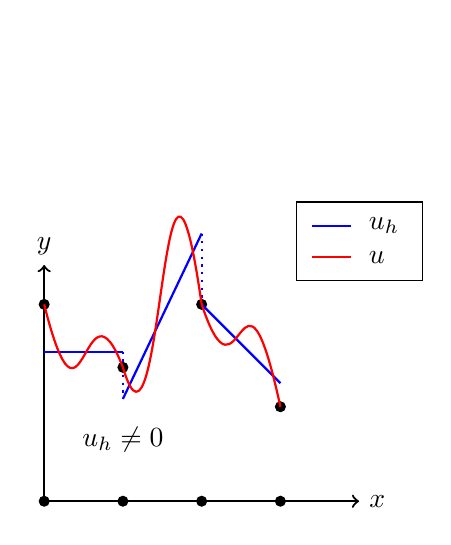
\begin{tikzpicture}
      % Draw x-axis
      \draw[->, thick] (0,0) -- (4,0) node[right] {$x$};
      % Draw y-axis
      \draw[->, thick] (0,0) -- (0,3) node[above] {$y$};

      % Draw nodes at center, A, B, and C with arbitrary y-values
      \foreach \x/\y in {0/2.5, 1/1.7, 2/2.5, 3/1.2} {
        \fill (\x,\y) circle (2pt); % Filled nodes with y-values
        \fill (\x,0) circle (2pt); % Filled circles on x-axis
      }

      % Draw discontinuous interpolation between points
      \draw[blue, thick] (0,1.9) -- (1,1.9);
      \draw[blue, thick] (1,1.3) -- (2,3.4);
      \draw[blue, thick] (2,2.5) -- (3,1.5);

      % Draw dotted lines between discontinuous interpolations
      \draw[blue, thick, dotted] (1,1.9) -- (1,1.3);
      \draw[blue, thick, dotted] (2,3.4) -- (2,2.5);

      \node at (1,0.5) [above] {$\jump{ u_{h} } \neq 0$};

      \draw[red, thick] (0,2.5) .. controls (0.5,0.5) and (0.5,3) .. (1,1.7) .. controls (1.5,0) and (1.5,6) .. (2,2.5) .. controls (2.5,1) and (2.5,3.5) .. (3,1.2);

      \draw (3.2,2.8) rectangle (4.8,3.8); % Legend box
      \draw[blue, thick] (3.4,3.5) -- (3.9,3.5); % Blue line for u_h
      \draw[red, thick] (3.4,3.1) -- (3.9,3.1); % Red line for u
      \node[anchor=west] at (4.0,3.5) {$u_h$}; % Label for u_h
      \node[anchor=west] at (4.0,3.1) {$u$}; % Label for u

    \end{tikzpicture}
    \caption{Illustration of locally discontinuous elements using $P^{1}$.}
    \label{fig:DG_P1_ements}
  \end{minipage}
\end{figure}

\begin{figure}
  \centering
  \begin{minipage}[b]{0.45\textwidth}
    \centering
    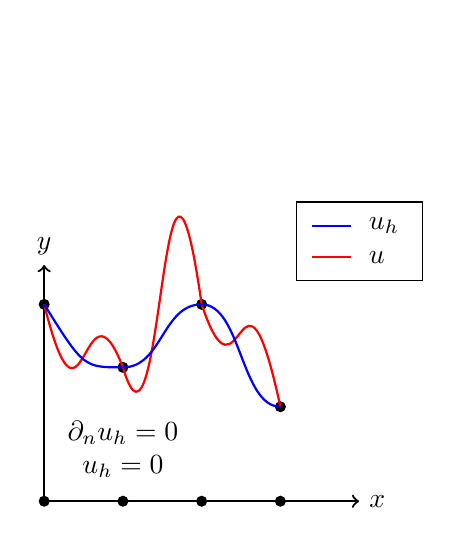
\begin{tikzpicture}
        % Draw x-axis
        \draw[->, thick] (0,0) -- (4,0) node[right] {$x$};
        % Draw y-axis
        \draw[->, thick] (0,0) -- (0,3) node[above] {$y$};

        % Draw nodes at center, A, B, and C with arbitrary y-values
        \foreach \x/\y in {0/2.5, 1/1.7, 2/2.5, 3/1.2} {
            \fill (\x,\y) circle (2pt); % Filled nodes with y-values
            \fill (\x,0) circle (2pt); % Filled circles on x-axis
        }

        % Exact solution
        \draw[red, thick] (0,2.5) .. controls (0.5,0.5) and (0.5,3) .. (1,1.7) .. controls (1.5,0) and (1.5,6) .. (2,2.5) .. controls (2.5,1) and (2.5,3.5) .. (3,1.2);
        \node at (1,0.6) [above] {$\jump{ \partial _{n} u_{h} } = 0$};
        \node at (1,0.7) [below] {$\jump{ u_{h} }   = 0$};

        % Second
        \draw[blue, thick] (0,2.5) .. controls (0.5,1.7) and (0.5,1.7) .. (1,1.7) .. controls (1.5,1.7) and (1.5,2.5) .. (2,2.5) .. controls (2.5,2.5) and (2.5,1.2) .. (3,1.2);

        \draw (3.2,2.8) rectangle (4.8,3.8); % Legend box
        \draw[blue, thick] (3.4,3.5) -- (3.9,3.5); % Blue line for u_h
        \draw[red, thick] (3.4,3.1) -- (3.9,3.1); % Red line for u
        \node[anchor=west] at (4.0,3.5) {$u_h$}; % Label for u_h
        \node[anchor=west] at (4.0,3.1) {$u$}; % Label for u

    \end{tikzpicture}
    \caption{Illustration of globally $C^{1}$ continuous elements using $P^{2}$ elements.}
    \label{fig:C1_P2_ements}
  \end{minipage}
  \hfill
  \begin{minipage}[b]{0.45\textwidth}
    \centering
    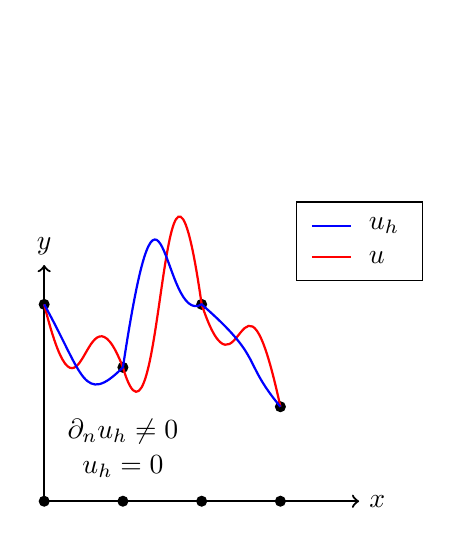
\begin{tikzpicture}
        % Draw x-axis
        \draw[->, thick] (0,0) -- (4,0) node[right] {$x$};
        % Draw y-axis
        \draw[->, thick] (0,0) -- (0,3) node[above] {$y$};

        % Draw nodes at center, A, B, and C with arbitrary y-values
        \foreach \x/\y in {0/2.5, 1/1.7, 2/2.5, 3/1.2} {
            \fill (\x,\y) circle (2pt); % Filled nodes with y-values
            \fill (\x,0) circle (2pt); % Filled circles on x-axis
        }

        % Exact solution
        \draw[red, thick] (0,2.5) .. controls (0.5,0.5) and (0.5,3) .. (1,1.7) .. controls (1.5,0) and (1.5,6) .. (2,2.5) .. controls (2.5,1) and (2.5,3.5) .. (3,1.2);
        \node at (1,0.6) [above] {$\jump{ \partial _{n} u_{h} } \neq 0$};
        \node at (1,0.7) [below] {$\jump{ u_{h} }   = 0$};

        % Second
        \draw[blue, thick] (0,2.5) .. controls (0.5,1.6) and (0.5,1.2) .. (1,1.7) .. controls (1.5,5.0) and (1.5,2.2) .. (2,2.5) .. controls (2.8,1.8) and (2.5,1.8) .. (3,1.2);

        \draw (3.2,2.8) rectangle (4.8,3.8); % Legend box
        \draw[blue, thick] (3.4,3.5) -- (3.9,3.5); % Blue line for u_h
        \draw[red, thick] (3.4,3.1) -- (3.9,3.1); % Red line for u
        \node[anchor=west] at (4.0,3.5) {$u_h$}; % Label for u_h
        \node[anchor=west] at (4.0,3.1) {$u$}; % Label for u

    \end{tikzpicture}
    \caption{Illustration of $C^{0}$ continuous elements and locally $C^1$ using $P^{2}$.}
    \label{fig:C0_P2_ements}
  \end{minipage}
\end{figure}


\todo[inline]{ Question? Why do we not use complete DG for biharmonic? }

The goal is to find a useful full weak formulation of \eqref{eq:bi_problem}. Now, let the solution space be on the form,
\begin{equation*}
V = \left\{ v \in H^2( \Omega  ) : \partial _{n} v = g_{1}    \text{ on }
\Gamma   \right\}.
\end{equation*}
Let $u,v \in  V$, then the derivation of the general weak form is,
\[
\begin{split}
\left( \Delta ^2 u,v \right) _{\Omega }  &  = \left( \partial _{n} \Delta u, v \right) _{\Gamma  } - \left( \nabla \left( \Delta  u \right) , \nabla v \right) _{\Omega }  \\
\end{split}
\]
In fact, the simplest formulation has the form,
\[
  \left( \nabla \left( \Delta u \right) , \nabla v \right) _{\Omega } =   \left( \Delta u, \partial _{n} v \right) _{\Gamma  } - \left( \Delta u, \Delta v \right)_{\Omega },
\]
A major issue with this formulation is that we do not have boundary condition for $\Delta u$. Instead, we can expand the term in the following fashion.

\begin{equation*}
    \begin{split}
\left( \nabla \left( \Delta u \right) , \nabla v \right) _{\Omega } & = \sum_{i = 1}^{ d}  \left( \Delta  \partial _{x_{i}} u, \partial _{x_{i}}v \right) _{\Omega }  \\
&= \sum_{i = 1}^{d}  \left( \nabla \cdot \left( \nabla \partial _{x_{i}} u \right) , \partial _{x_{i}} v \right)_{\Omega }  \\
&= \sum_{i = 1}^{d}  \left( \partial_n  \partial _{x_{i}} u, \nabla  \partial _{x_{i}} v \right) _{\Gamma } -   \left( \nabla \partial _{x_{i}} u, \nabla \partial _{x_{i}} v \right)_{\Omega }  \\
&= \left(  \partial_n\nabla u, \nabla v \right) _{\Gamma  } - \left( D^2 u, D^2v \right) _{\Omega } \\
&= \left( \partial _{nn} u, \partial _{n} v  \right)_{\Gamma  }   + \left( \partial _{nt} u, \partial _{t} v \right) _{\Gamma  } - \left( D^2u, D^2v \right) _{\Omega } .
    \end{split}
.\end{equation*}
Hence, the boundary condition of $\Delta u$ is integrated into the formulation.  It can be denoted that $D^2$ is the Hessian matrix operator s.t.
$$( D^2u, D^2v )_{\Omega } = \int_{\Omega }^{} D^{2}u : D^2v  dx,$$
where $D^2u:D^2v$ is the inner product and similarly for $\partial _{nn} u = n\cdot D^2 u \cdot n$. Thus, we now have a weak form identity,
\begin{equation}
\label{eq:weak_form_identity}
\left( \Delta ^2 u, v \right) _{ \Omega } = \left( D^2u, D^2v \right) _{\Omega} +   \left( \partial _{n} \Delta u, v  \right) _{\Gamma  }  - (\partial _{nn} u, \partial _{n} v )_{\Gamma  } - \left( \partial _{nt} u, \partial _{t}v
\right) _{\Gamma  }
.\end{equation}

Using weak form identity \eqref{eq:weak_form_identity} and the boundary conditions stated in the strong form \eqref{eq:bi_problem} can we write

\begin{equation}
\begin{split}
\left( \Delta ^2 u, v \right) _{ \Omega } & = \left( D^2u, D^2v \right) _{\Omega} +   \underbrace{\left( \partial _{n} \Delta u, v  \right) _{\Gamma  }}_{ = \left( g_{2},v \right) _{\Gamma  }}   - \underbrace{(\partial _{nn} u, \partial
    _{n} v )_{\Gamma  }}_{ = 0}  - \underbrace{\left( \partial _{nt} u, \partial _{t}v \right) _{\Gamma  }}_{ = 0} \\
    &= \left( D^2u, D^2v \right) _{\Omega } + \left( g_{2},v \right) _{\Gamma  }  \\
\end{split}
.\end{equation}
\todo[inline]{ Is it a way to prove $\partial _{nn} u = 0$ and $\partial _{nt} u = 0$ on $\Gamma  $? }

Finally, we can define the following bilinear functional $a:V\times V \to  \mathbb{R} $ and the linear functional $F: V \to \mathbb{R} $ s.t.
\begin{equation}
\label{eq:weak_formulation}
\begin{split}
a\left( u,v \right) & =    \left( D ^2 u , D ^2 v\right)_{\Omega }  +
\alpha \left( u, v \right)_{\Omega }   , \\
l\left( v \right) & = \left( f,v \right)_{\Omega } - \left(g_{2},v \right)_{\partial \Omega }.
\end{split}
\end{equation}

Thus, we have now the necessary definitions to define the biharmonic problem.

We define the biharmonic problem to solve for $u \in V  $ s.t.
\begin{equation}
    \label{eq:bi_weak1}
a\left( u,v \right) = l(v)\quad \forall v \in
V,
\end{equation}
where $ V = \left\{ v \in H^2\left( \Omega  \right) : \partial _{n} v = g_{1}  \text{ on }
\Gamma   \right\}$.

Remark that the problem the solution is only unique for $\alpha  > 0$. However, for $\alpha  = 0$ is it necessary to apply the solvability condition,
\begin{equation*}
 \int_{\Omega }^{} f dx = \int_{\Gamma  }^{} g ds
.\end{equation*}
This condition easily arise when using the substitution $v=1$ in \eqref{eq:bi_weak1}. To handle this, can we extended the solution space \[
V^{*} = \begin{cases}
    V \quad & \alpha  > 0 \\
    \left\{ v \in V: \int_{\Omega }^{} v dx  = 0\right\} \quad & \alpha  = 0,
\end{cases}
\]
However, we will from now generally assume that $\alpha >0$.
Thus, the unique solution in $v \in V^{*}$ belongs to $H^{3 }(\Omega ) $ and we get the following
elliptic regularity estimate \cite{gu2012c0},
\begin{equation*}
\label{eq:bi_harmonic_ellitpic_regularity}
\left| u \right| _{H^{3 }\left( \Omega  \right) }  \le C_{\Omega } \left( \| f \|_{  L^{2}( \Omega ) }^{  } + ( 1 + \alpha  ^{\frac{1}{2}}
) \cdot \| w  \|_{ H^{4}\left( \Omega  \right)  }^{  }    \right) \quad w\in H^{4}\left( \Omega  \right).
\end{equation*}

Finally, we can define the complete weak formulation of the biharmonic problem.
We define the biharmonic problem to find $u \in V^*  $ s.t.
\begin{equation}
a\left( u,v \right) = l(v)\quad \forall v \in
V^* .
\end{equation}

\subsection{Constructing Continuous Interior Penalty Method}%
\label{sub:constructing_continious_interior_penalty_method}

 Let us assume that $u,v \in
H^{4}\left( T  \right) $. Using that the weak form identity \eqref{eq:weak_form_identity} also holds for a triangle $T$ can we write
\begin{equation}
\label{eq:bi_basic_dg}
\left( \Delta  ^{2} u,v \right) _{T} =  \left( D^2u,D^2v \right) _{T } - \left(\partial _{nt} u, \partial _{t}v
\right)_{\partial T} - \left(\partial _{nn} u, \partial _{n}v \right)_{\partial T} + \left(\partial _{n} \Delta  u,v
\right)_{\partial T}
.\end{equation}
For global continuity, let  $v \in V =  \left\{ v \in H^{1}\left( \Omega  \right): v_{T} \in  H^{4}\left( T \right), \ \forall T \in
\mathcal{T}_{h}    \right\} $ and $u \in  H^{4}\left( \Omega  \right) $ such that,

\begin{equation}
\label{eq:bi_basic_dg2}
\left( \Delta  ^{2} u,v \right) _{\Omega } = \sum_{T \in  \mathcal{T} _{h}}^{}  \left( D^2u,D^2v \right) _{T } - \left(\partial _{nt} u, \partial _{t}v
\right)_{\partial T} - \left(\partial _{nn} u, \partial _{n}v \right)_{\partial T} + \left(\partial _{n} \Delta  u,v
\right)_{\partial T}.
\end{equation}
However, this expression can be written to distinguish integrating over triangles $\mathcal{T} _{h}$ , integrating over exterior facets $\mathcal{F} _{h}^{ext}$ and then integrate interior facets $\mathcal{F} _{h}^{int}$.

\begin{equation}
\label{eq:bi_basic_dg_full_1}
\begin{split}
\left( \Delta  ^{2} u, v \right) _{\Omega } =& \sum_{T \in  \mathcal{T} _{h}}^{} \left( D^2u, D^2v \right)_{T}    \\
& + \sum_{F \in \mathcal{F}_{h}^{ext}}  \left(\partial _{n} \Delta u, v  \right) _{F} - \left(\partial _{nt} u, \partial _{t} v \right) _{F}-
\left( \partial _{nn} u, \partial _{n} v \right)_{F}  \\
& + \sum_{F \in \mathcal{F}_{h}  ^{int}}^{} \left(\partial _{nn} u , \jump{ \partial _{n} v }
\right)_{F} \\
& = \sum_{T \in  \mathcal{T} _{h}}^{} \left( D^2u, D^2v \right)_{T} + \sum_{F \in
\mathcal{F} ^{ext}_{h}}^{} \left(g_{2}, v  \right) _{F}
  + \sum_{F \in \mathcal{F}_{h}  ^{int}}^{} \left( \partial _{nn} u , \jump{ \partial_{n} v } \right)_{F}
\end{split}
\end{equation}
Keep in mind that any jump over a interior facet $F \subset \mathcal{F} _{h}^{int}   $, visualized in figure \ref{fig:normal}, is defined as $\jump{ a } =    a^{+} - a^{-} $
and likewise for the mean, $\mean{ a  } = \frac{1}{2}(   a^{+}
+ a^{-})$.    The equivalence of \eqref{eq:bi_basic_dg2} and \eqref{eq:bi_basic_dg_full_1} comes from the following argumentation.

\begin{equation*}
    \begin{split}
 \left( \Delta  ^{2} u,v \right) _{\Omega } & =\sum_{T\in \mathcal{T} _{h}}^{} \left( D^2u,D^2v \right) _{T } - \left(\partial _{nt} u, \partial _{t}v
\right)_{\partial T} - \left(\partial _{nn} u, \partial _{n}v \right)_{\partial T} + \left(\partial _{n} \Delta  u,v
\right)_{\partial T} \\
&= \sum_{T\in \mathcal{T} _{h}}^{} \left( D^2u,D^2v \right) _{T } \\
&  \quad + \sum_{F \in \mathcal{F}_{h}^{ext} }^{} \underbrace{\left( \partial _{n} \Delta  u, v  \right)_{F}}_{= \left( g_{2},v \right)_{F} }  -  \left(
\partial _{nt} u, \partial _{t} v \right) _{F}  - \underbrace{\left( \partial _{nn} u, \partial _{n} v \right)_{F}}_{ = 0}    \\
& \quad  + \sum_{F \in \mathcal{F} _{h}^{int}}^{} \underbrace{\left( \left(\partial _{n^{+}} \Delta  u^{+}
        ,v^{+}\right)_{F}
+ \left(\partial _{n^{-}} \Delta  u^{+} ,v^{-}\right)_{F}  \right)}_{(I)} \\
 & \quad \quad \quad  \quad +
\underbrace{\left( \left(\partial _{n^{+}t} u^{+}, \partial_{t} v^{+} \right)_{F} +  \left(\partial _{n^{-}t} u^{-},
        \partial_{t} v^{-}
\right)_{F}  \right) }_{(II)} \\
 & \quad \quad \quad  \quad  +
\underbrace{\left( \left(\partial _{n^{+}n^{+}} u^{+}, v^{+} \right) _{F} + \left(\partial _{n^{-}n^{-}} u^{-}, v^{-}
\right) _{F} \right) }_{(III)}
    \end{split}
.\end{equation*}

Where integration over all interior facets $ \forall F \in \mathcal{F}_{h}^{int}$ is computed in this way.
\begin{equation*}
    \begin{split}
        (I) &  =    \left(\partial _{n^{+}} \Delta  u^{+} ,v^{+}\right)_{F} +
        \left(\partial _{n^{-}} \Delta  u^{-} ,v^{-}\right)_{F}  \\
        & =   \int_{F}^{}
        \jump{ \partial _{n} \Delta  u \cdot v } =
         \int_{F}^{}
         \mean{ \partial _{n} \Delta  u } \underbrace{\jump{ v }}_{= 0}    + \underbrace{\jump{ \partial _{n} \Delta  u
         }}_{= 0}    \mean{ v } = 0 \\
        (II) &  =     \left(\partial _{n^{+}t} u^{+}, \partial_{t} v^{+}
        \right)_{F} +  \left(\partial _{n^{-}t} u^{-}, \partial_{t} v^{-}
\right)_{F}   \\
&  =   \int_{F}^{}
        \jump{ \partial _{nt} u \cdot  \partial_{t} v } =
         \int_{F}^{}
         \mean{ \partial _{nt} u    } \underbrace{\jump{ \partial_{t} v }  }_{= 0}    + \underbrace{\jump{ \partial
                 _{nt}  u
         }}_{= 0}    \mean{ \partial _{t}v }  = 0\\
        (III) &  =     \left(\partial _{n^{+}n^{+}} u^{+}, \partial_{n^{+}} v^{+} \right)_{F} +  \left(\partial _{n^{-}n^{-}} u^{-}, \partial_{n^{-}} v^{-} \right)_{F}    =    \int_{F}^{} \jump{ \partial _{nn} u \cdot  \partial_{n} v }  \\
        & = \int_{F}^{}
        \mean{ \partial _{nn} u    } \underbrace{\jump{ \partial_{n} v }  }_{\neq 0}    + \underbrace{\jump{ \partial
                 _{nn}  u
         }}_{= 0}    \mean{ \partial _{n}v }   =  \left( \partial _{nn} u, \jump{ \partial_{n} v } \right)_{F}   \end{split}
.\end{equation*}
Observe that the cancellations in the term $(I)$ appears of the continuity of $v\in V $ and $u\in H^{4}( \Omega ) $ which makes the jumps zero. For the second term $(II)$ does the terms become zero cancelled because the tangential
derivative at the facet has no jump. However, The third term $(III)$  is fairly interesting since the discontinuity in
normal vector for $v \in V$ is a jump, while the second term is still continuous. It can also be raised that $\mean{
\partial _{nn} u } = \partial _{nn} u  $ holds by the continuity of $H^{4}( \Omega  ) $. Hence,
\eqref{eq:bi_basic_dg2} and \eqref{eq:bi_basic_dg_full_1} is equivalent.

\subsection{Formulation of the Continuous Interior Penalty Method}%
\label{sub:formulation_of_continious_interior_penalty_method}


We can finally start defining the fully discrete formulation. Let the basis be a $\mathcal{P}_{2} $ Lagrange finite element space so,
\[
V_{h} = \left\{ v \in C^{0}\left( \Omega  \right): v_{T} = v | _{T} \in \mathcal{P} _{2}\left( T \right), \forall T \in
\mathcal{T}_{h}    \right\}
\]
and
\[
V_{h}^{*} = \begin{cases}
    V_{h} & \text{ if } \alpha  > 0 \\
    \left\{ v \in V_{h}: \int_{\Omega }^{} v dx   = 0   \right\} &  \text{ if } \alpha   = 0
\end{cases}
\]
Now, if we choose $u \in V_{h}$, then we must take account that the jump is discrete.
 Finally, the CIP formulation can be stated as follows.
The discretized numerical problem is to solve $w \in V_{h}^{*}$ such that
\begin{equation}
\label{eq:CP_A_F}
a_{h}( w, v )   = l_{h}( v), \quad \forall v \in V_{h}^{*}  .
\end{equation}
where
\begin{equation}
\label{eq:CP_A_h_1}
\begin{split}
a_{h} ( w, v )   =&
    \left( \alpha  w, v \right) _{\Omega } + \sum_{T \in \mathcal{T} _{h}}^{} \left( D^2 w, D^2v \right) _{T} \\
 & + \sum_{F \in \mathcal{F}_{h} }^{}
  \left( \mean{  \partial _{n n} w }, \jump{ \partial _{n }v} \right)_{F}  +
 \left( \mean{ \partial _{n n} v }, \jump{ \partial _{n}w }      \right)_{F}   + \frac{\gamma}{h}  \left( \jump{ \partial _{n} w}, \jump{ \partial _{n} v   }   \right)_{F}
\end{split}
\end{equation}
and
\begin{equation}
\label{eq:CP_F_h}
l_{h}( v )  = \left( f, v \right) _{\Omega } +  \sum_ {F \in \mathcal{F}_{h} ^{ext}}^{} - \left(g_{2}, v  \right) _{F}.
\end{equation}
Notice that the regulation term determined by respectively a global tuning parameter $\gamma >0 $. Another key component to the formulation
in \eqref{eq:CP_A_h_1} after introduction of $ w, v \in V^{*}_{h}$  is that we expanded $\left( \partial _{nn}w, \jump{ \partial _{n} v }  \right)_{F} \to \left( \mean{ \partial _{nn}w }  , \jump{ \partial _{n} v }  \right)_{F} $ since we can longer not guarantee a
continuous jump. For symmetric purposes we also added $ \left( \mean{ \partial _{nn} v}  , \jump{ \partial _{n} w }  \right)_{F} $. For convenience will we introduce the compact notation of \eqref{eq:CP_A_h_1} and \eqref{eq:CP_F_h};

\begin{equation*}
\begin{split}
a_{h} \left( w, v \right)   =&
    \left( \alpha  w, v \right) _{\Omega }   +  \left( D^2 w, D^2v \right) _{\mathcal{T} _{h}} \\
 & +
  \left( \mean{  \partial _{n n} w }, \jump{ \partial _{n }v} \right)_{\mathcal{F}_{h}}  +
 \left( \mean{ \partial _{n n} v }, \jump{ \partial _{n}w }      \right)_{\mathcal{F}_{h}}  + \frac{\gamma }{h}  \left( \jump{ \partial _{n} w}, \jump{ \partial _{n} v   }   \right)_{\mathcal{F}_{h}} \\
 l_{h}( v_{h}) & =  \left( f, v \right) _{\Omega }  - \left(g_{2}, v  \right) _{\Gamma }
\end{split}
\end{equation*}


\subsection{Note on the Biharmonic Mixed Formulation}%
\label{subsec:biharmonic_mixed_formulation}

It is easy to see that the biharmonic problem can be rewritten into an equivalent mixed formulation , that is, to find $\sigma, \tau  \in H^2( \Omega ) $ s.t. \[
    \begin{split}
\Delta \sigma  & = f \quad  \text{in } \Omega \\
\sigma   & = \Delta u  \text{ in } \Omega \\
\partial _{n} \sigma  & = g_{1} \text{ on } \Gamma  \\
\partial _{n} u   & = g_{2} \text{ on } \Gamma
    \end{split}
\]
The goal is to obtain an useful weak formulation. Using Greens theorem on the first equation we get,
\[
( \sigma, v)_{\Omega } = ( \nabla  u , \nabla v  )_{\Omega } - ( \nabla _{n} u , v) _{\Gamma }.
\]
Similarly for the second equation we obtain
\[
( \nabla \sigma , \nabla \varphi  )_{\Omega} - ( \nabla _{n} \sigma ,  \varphi )_{\Gamma } = ( f,\varphi ) _{\Omega}
\]
Putting it all together we have the following mixed weak formulation; Find $( u, \sigma ) \in H^{1}( \Omega ) \times H^{1}( \Omega )  $ s.t. \[
    \begin{split}
     ( \nabla  u , \nabla v  )_{\Omega } -( \sigma, v)_{\Omega }  & =   ( g_{1} , v) _{\Gamma } \quad  \forall v \in H^{1}( \Omega ) \\
( \nabla \sigma , \nabla \varphi  )_{\Omega}  & = ( f,\varphi ) _{\Omega} + ( g_{2} ,  \varphi )_{\Gamma } \quad  \forall \varphi \in H^{1}( \Omega )
    \end{split}
\]
Now we want to relate this formulation to the abstract saddle point problem (SPP) (find references).
Let $V = H^{1}( \Omega ) $  and $W=H^{1}( \Omega ) $ be  Hilbert spaces and define the bilinear form $a: V\times V \to \mathbb{R}  $ and $b: V \times W \to \mathbb{R} $ s.t. $a( \sigma,v ) = - ( \sigma , v) _{\Omega }  $ and $b( u,v) = ( \nabla u,
\nabla v)_{\Omega  }  $. We also may define the linear forms, $G,F: V \to \mathbb{R} $ s.t. $ G( v)  = ( g_{1}, v) _{\Gamma } $ and $F( \varphi ) = ( f, \varphi )_{\Omega } + ( g_{2}, \varphi )_{\Gamma } $.

Hence, we can connect it to the SPP. We want to find $( u,\sigma ) \in V \times W$ s.t.  \[
    \begin{cases}
       a( \sigma ,v) + b ( u, v )  & = G( v)   \quad  \forall v \in V \\
       b( u, \varphi  )  & = F( \varphi )     \quad \forall \phi \in W
    \end{cases}
\]
This is useful since we can now apply standard saddle point theory to do an analysis for the problem. We will see that it is now easier to handle the constraints with the cost of a more challenging time discretization step when applying the formulation to the Cahn-Hilliard Problem.
A well known and mature application for SPP is the well known Stokes equation \cite{john2016finite, knabner2003numerical}. One of the more classical papers for the biharmonic mixed formulation is and still in active research going on \cite{babuvska1980analysis,cai2023nitsche}.

However, in this master thesis is the focus on solving the biharmonic equation avoiding the mixed formulation using the CIP formulation, which does in fact handle the downsides with the SPP problem.


